% Created 2026-04-23 Thu 12:09
% Intended LaTeX compiler: lualatex
\DocumentMetadata{lang = en-US,pdfversion = 2.0,pdfstandard = ua-2,tagging = on,tagging-setup = {math/setup=mathml-SE},}
\documentclass[11pt]{article}
\usepackage{amsmath}
\usepackage{fontspec}
\usepackage{graphicx}
\usepackage{longtable}
\usepackage{wrapfig}
\usepackage{rotating}
\usepackage[normalem]{ulem}
\usepackage{capt-of}
\usepackage{hyperref}
\usepackage[margin=1in]{geometry}
\usepackage{fontspec}
\usepackage{verbatim, multicol, tabularx,}
\usepackage{amsmath, amsthm, amssymb, stmaryrd, latexsym, bm, listings, qtree}
\usepackage{framed}
\usepackage{xcolor,colortbl}
\usepackage{media9}
\usepackage[export]{adjustbox}
\usepackage{algorithm}
\usepackage[noend]{algpseudocode}
\usepackage{tikz,pgfplots}
\usetikzlibrary{shapes.geometric}
\let\oldquote=\quote
\let\endoldquote=\endquote
\colorlet{shadecolor}{cyan!15}
\renewenvironment{quote}{\begin{shaded*}\begin{oldquote}}{\end{oldquote}\end{shaded*}}
% From https://tex.stackexchange.com/questions/7032/good-way-to-make-textcircled-numbers
\newcommand*\circled[1]{\tikz[baseline=(char.base)]{\node[shape=circle,draw,inner sep=2pt] (char) {#1};}}
\DeclareMathOperator*{\argmin}{arg\!min}
\DeclareMathOperator*{\argmax}{arg\!max}
\lstset{frame=tb, aboveskip=1mm, belowskip=0mm, showstringspaces=false, columns=flexible, basicstyle={\scriptsize\ttfamily}, numbers=left, frame=single, breaklines=true, breakatwhitespace=true}
\hypersetup{colorlinks=true,urlcolor=blue}
\usepackage{tagpdf}
\tagpdfsetup{activate-all}
\tagpdfsetup{math/alt/use}
\usepackage{polyglossia}
\setdefaultlanguage[variant=en-US]{english}
\author{Christopher Simpkins}
\date{Kennesaw State University}
\title{Artificial Intelligence\\\medskip
\large Uncertainty}
\hypersetup{
 pdfauthor={Christopher Simpkins},
 pdftitle={Artificial Intelligence},
 pdfkeywords={},
 pdfsubject={Artificial Intelligence Uncertainty},
 pdfcreator={Emacs 30.2 (Org mode 9.7.11)}, 
 pdflang={English}}
\begin{document}

\maketitle
\section{From Logic to Probability Theory}
\label{sec:orgb4215f7}

Consider:

\begin{equation*}
Toothacke \implies Cavity
\end{equation*}

Not all patients with toothaches have cavities.  How about:

\begin{equation*}
Toothache \implies Cavity \lor GumProblem \lor Abscess \dots
\end{equation*}

We'd need large list after the dots.  Try causal direction:

\begin{equation*}
Cavity \implies Toothache
\end{equation*}

But not all cavities hurt.  Logic fails to deal with complex domains like medical diagonosis due to:

\begin{itemize}
\item \textbf{Exhaustivity} (laziness).  Too many antecedents or consequents to list.
\item \textbf{Theoretical ignorance}. Rare to have complete logical theory of nontrivial domain.
\item \textbf{Practical ignorance}.  Even with a complete domain theory, hard to measure all the necessary inputs (medical tests, etc.)
\end{itemize}

We need to deal with uncertain knowledge, with \textbf{degrees of belief}.  For that, we use probability theory.
\section{What do probabilities mean?}
\label{sec:orgab0386a}


\includegraphics[alt={neo architect prob dist screens},width=0.75\linewidth]{neo-architect-prob-dist-screens.png}
\section{What do probabilities mean?}
\label{sec:org912ce61}

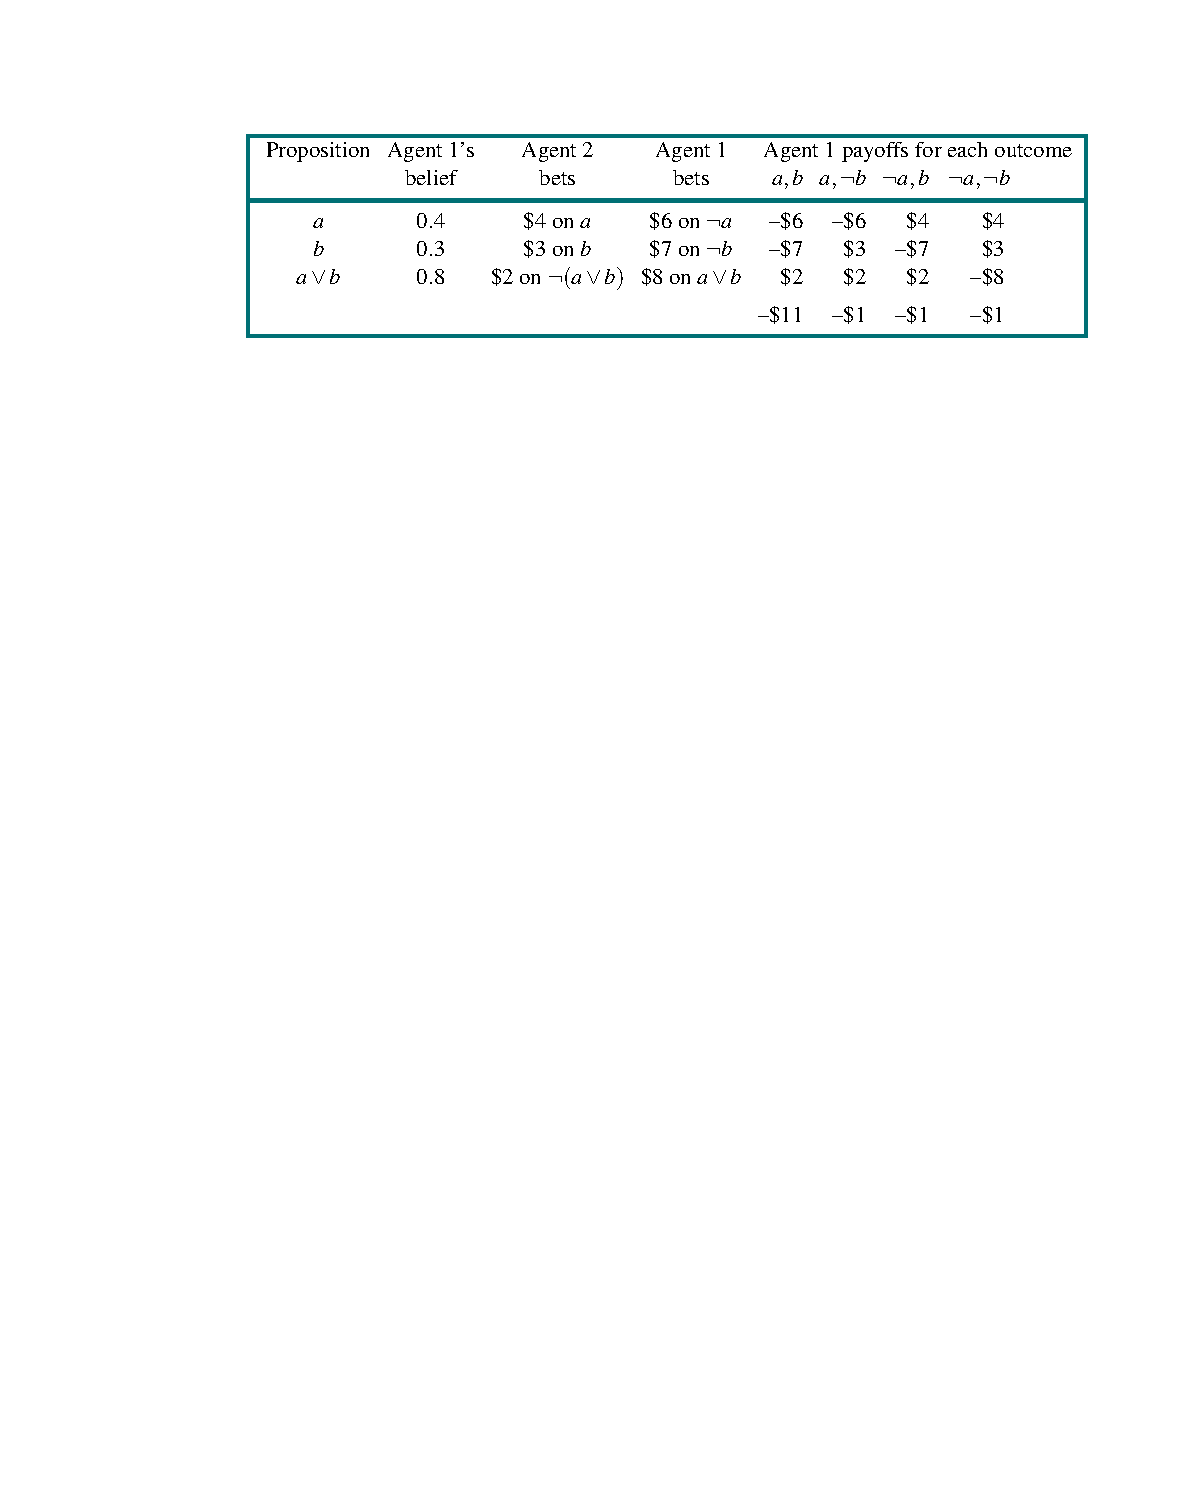
\includegraphics[alt={aima fig 12_02 agent bets},width=0.75\linewidth]{aima-fig-12_02-agent-bets.pdf}

All I see is the \texttt{code}.

\begin{lstlisting}[language=Python,numbers=none]
this_is = a_python_code_block
if it_is_not_processed:
    it_is_likely_within_a_column_env
    if not_in_colmn_env:
        there_is_another_problem
\end{lstlisting}
\section{Probabilities are about our uncertain knowledge.}
\label{sec:org4f8d885}

"80\% chance (probability 0.8) patient with a toothache has a cavity."

\begin{itemize}
\item Out of all the situations that are indistinguishable from the current situation \textbf{as far as our knowledge goes}, the patient will have a cavity in 80\% of them.
\item Belief could come from statistical data, or domain theory, or combination of sources.
\end{itemize}

\begin{quote}
There is no uncertainty in the actual world.  The patient either has a cavity or does not. Probabilities refer to our knowledge of the world state, not the actual world state.[\textsuperscript{fn}]
\end{quote}

If our knowledge changes, e.g., we find out patient has history of gum disease, we make a different statement. Here is a .

"Given patient has a history of gum disease and a toothache, 40\% chance patient has gum disease."

{[}\textsuperscript{fn}]: Footnote
{[}\textsuperscript{fn2}]: \url{https://this/isn't/real}
\section{Decision-Theoretic Agents}
\label{sec:org5bf3a08}

\begin{quote}
Decision theory = probability theory + utility theory
\end{quote}


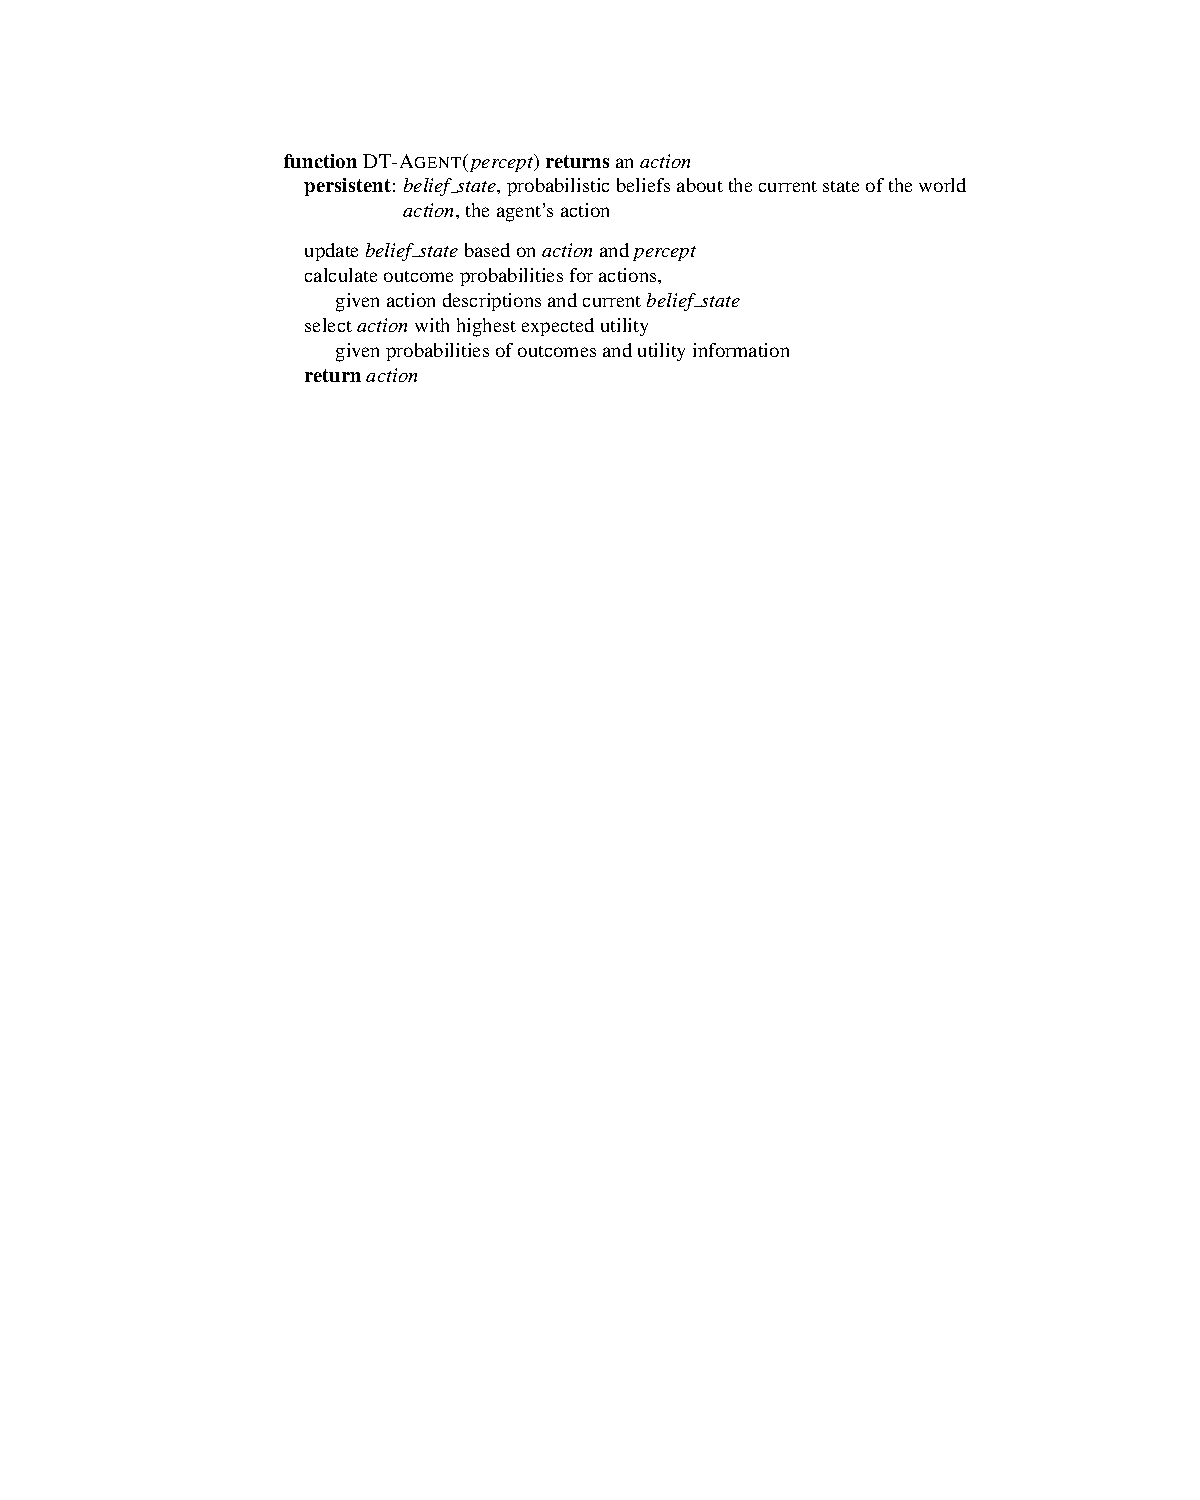
\includegraphics[alt={aima fig 12_01 dt agent algorithm},width=0.75\linewidth]{aima-fig-12_01-dt-agent-algorithm.pdf}


Each action, \(a\), leads to a probability distribution over outcomes, or "result states":

$$
P(\text{RESULT}(a) = s') = \sum_{s \in S} P(s) P(s' \mid s, a)
$$

And each outcome state has a utility.  A rational decision-theoretic agent chooses the action that maximize expected utility, that is:

$$
\argmax_{a} \sum_{s' \in S} P(\text{RESULT}(a) = s') U(s')
$$
\section{Propositions and Events}
\label{sec:org131a00a}

An \textbf{event}, which we denote with \(\phi\) here, is a set of possible worlds, some subset of \(\Omega\), or set of \(\omega\), e.g., the event "doubles" contains the 6 boxed elements \(\omega\):

\footnotesize
\tagpdfsetup\{table/header-rows=\{1\}\}
\begin{tabular}{cccccc}
\boxed{(1, 1)} & (2, 1) & (3, 1) & (4, 1) & (5, 1) & (6, 1)\\
(1, 2) & \boxed{(2, 2)} & (3, 2) & (4, 2) & (5, 2) & (6, 2)\\
(1, 3) & (2, 3) & \boxed{(3, 3)} & (4, 3) & (5, 3) & (6, 3)\\
(1, 4) & (2, 4) & (3, 4) & \boxed{(4, 4)} & (5, 4) & (6, 4)\\
(1, 5) & (2, 5) & (3, 5) & (4, 5) & \boxed{(5, 5)} & (6, 5)\\
(1, 6) & (2, 6) & (3, 6) & (4, 6) & (5, 6) & \boxed{(6, 6)}\\
\end{tabular}
\normalsize
\section{Analysis of Medical Screening Example}
\label{sec:org27367f9}





\begin{align*}
P(C=1)     &= \frac{1}{100} \\
P(C=0)     &= \frac{99}{100}\\
P(T=1 \mid C=1) &= \frac{90}{100}\\
P(T=0 \mid C=1) &= \frac{10}{100}\\
P(T=1 \mid C=0) &= \frac{3}{100} \\
P(T=0 \mid C=0) &= \frac{97}{100}
\end{align*}




If we screen someone, probability that they test positive (notice use of product rule: \(P(a, b) = P(a \mid b) P(b)\) and rule 2nd Kolmogorov axiom \(P(x \lor y) = P(x) + P(y) - P(x \land y)\)):

\vspace{-.1in}
\begin{align*}
P(T=1) &= P(T=1 \mid C=0)P(C=0) + P(T=1 \mid C=1)P(C=1)\\
       &= \frac{3}{100} \times \frac{99}{100} + \frac{90}{100} \times \frac{1}{100}\\
       &= \frac{387}{10,000}\\
       &= .0387
\end{align*}

If someone tests positive, probability they have cancer :
\end{document}
